\chapter{Programme of the tournament}

\begin{enumerate}
\item The number of participants in the tournament is limited to twenty, of whom one half are Russian players.

\item Every participant meets every one of his competitors in one game. A game won counts Plus One, a game lost counts Naught, and a draw one half a point.

%%%%%%%%%%%%%%%%
\begin{figure}[h]
\centering
\sc{in the first round}\\
\vspace{0.1cm}
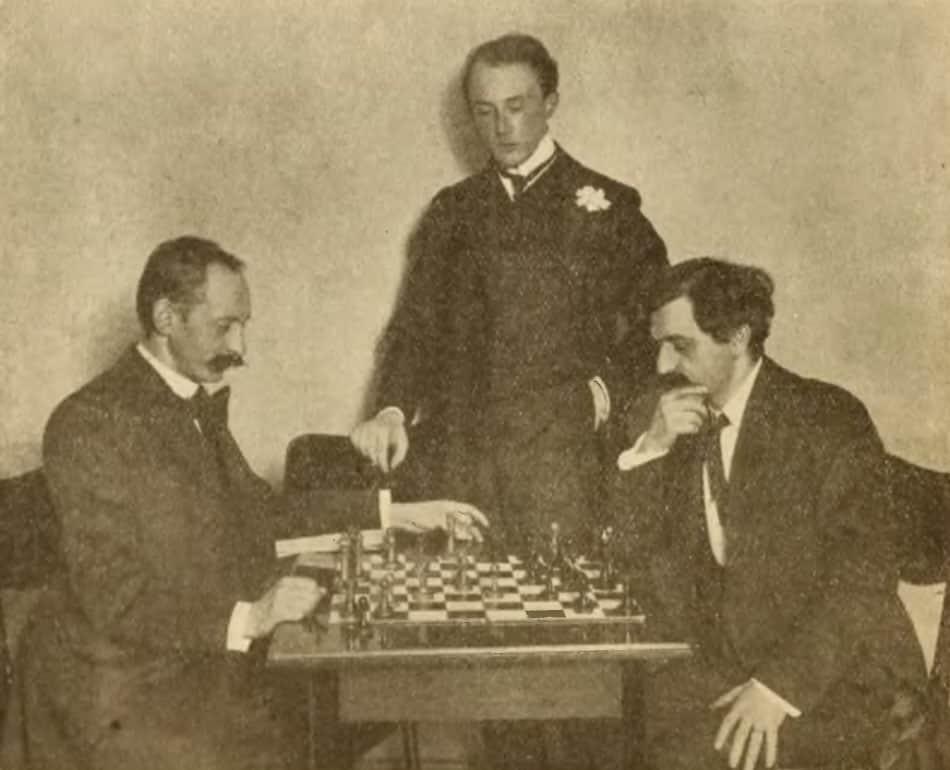
\includegraphics[width=\textwidth]
{img/i1_schlecter-lasker.jpg}\\
\small
c.~schlecter \hspace{5cm} dr e.~lasker
\end{figure}
%%%%%%%%%%%%%%%%

\item No entrance fee is necessary, but a deposit of 10 Rbls. is demanded. It shall be paid before the commencement of the tournament and is repaid provided the participant has stayed in the tournament until the end.

\item Ten prizes: - I, 1000 Rbls.~(a little more than \$500.00 or \pounds 100) ; II, 750 Rbls.~; III, 550; IV, 400; V, 280; VI, 190; VII, 120; VIII, 80; IX, 50; X, 30.

%%%%%%%%%%%%%%%%
\begin{figure}[h]
\centering
\sc{tournament committee members}\\
\vspace{0.1cm}
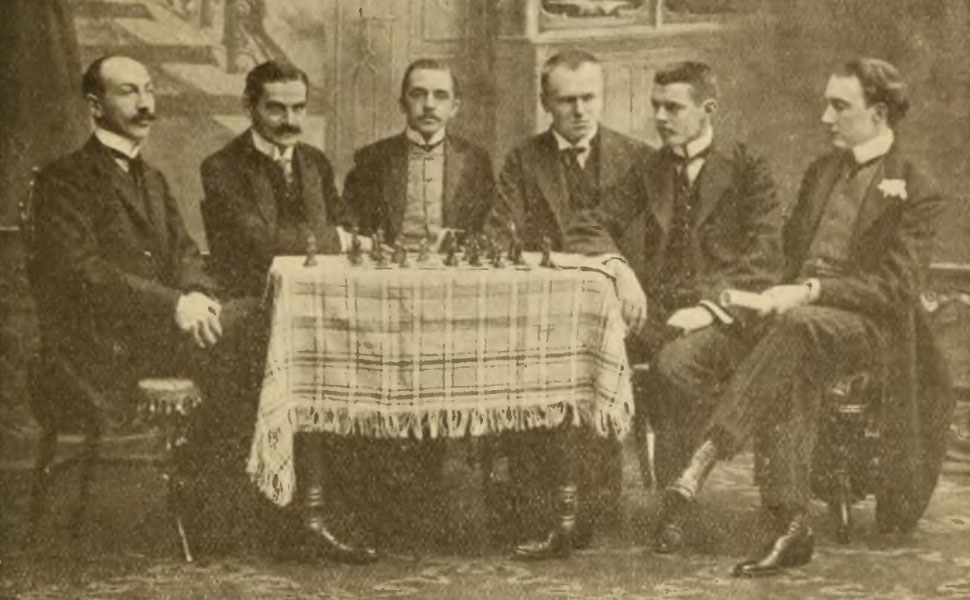
\includegraphics[width=\textwidth]
{img/i2_committee-members.jpg}\\
\small
b.~maljutin, o.~sossnitzky, s.znosko--borovsky, p.~p.~saburov, e.~a.~znosko--borovsky, v.~tschudowski
\end{figure}
%%%%%%%%%%%%%%%%

\item All participants receive also an honorary of 10 Rbls.~for each game they win and 5 Rbls.~for each game they draw.

\item Furthermore, each competitor receives a fixed compensation. Every Russian Master 50 Rbls., and every foreign participant 100 Rbls.

\item If the scores are equal the prizes are equally divided, except that two participants compete for the two first prizes. The two competitors agreeing, they can decide the first prize by a match of tour games. If the result should be equal the two prizes are divided.

\item Time for playing is five times a week, from 11 o'clock A.M.~until 9 o'clock P.M.~with an interval from 4 to 6 o'clock P.M. Before the adjournment the player whose turn it is to move must give his move in a closed envelope to the director of the tournament. The sixth day is reserved for the termination of adjourned games. Adjourned games may also be played, the two opponents agreeing, on any evening after the termination of other games which they might have to play. One day a week is an off day.

%%%%%%%%%%%%%%%%
\begin{figure}[h]
\centering
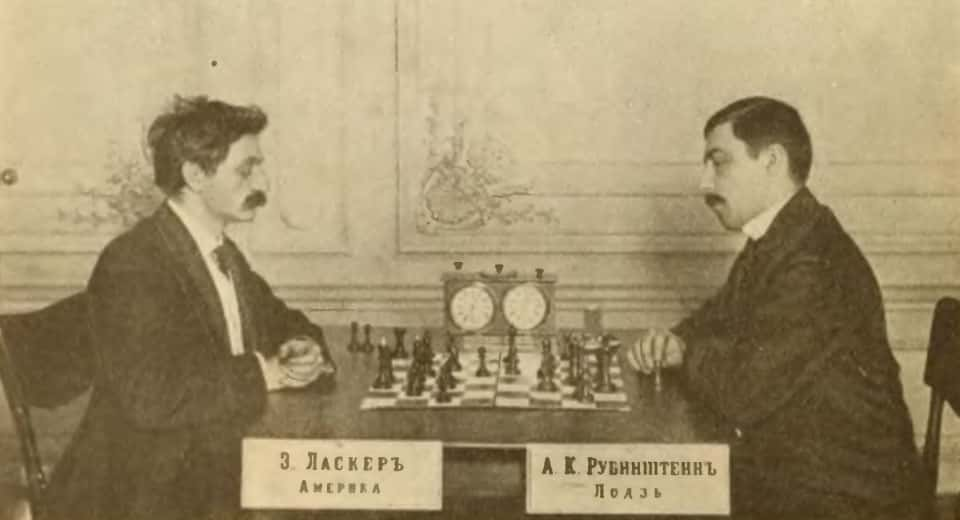
\includegraphics[width=\textwidth]
{img/i3_lasker-rubinstein.jpg}\\
\small\sc
dr e.~lasker \hspace{5cm} a.~k.~rubinstein
\end{figure}
%%%%%%%%%%%%%%%%

%%%%%%%%%%%%%%%%
\begin{figure}[h]
\centering
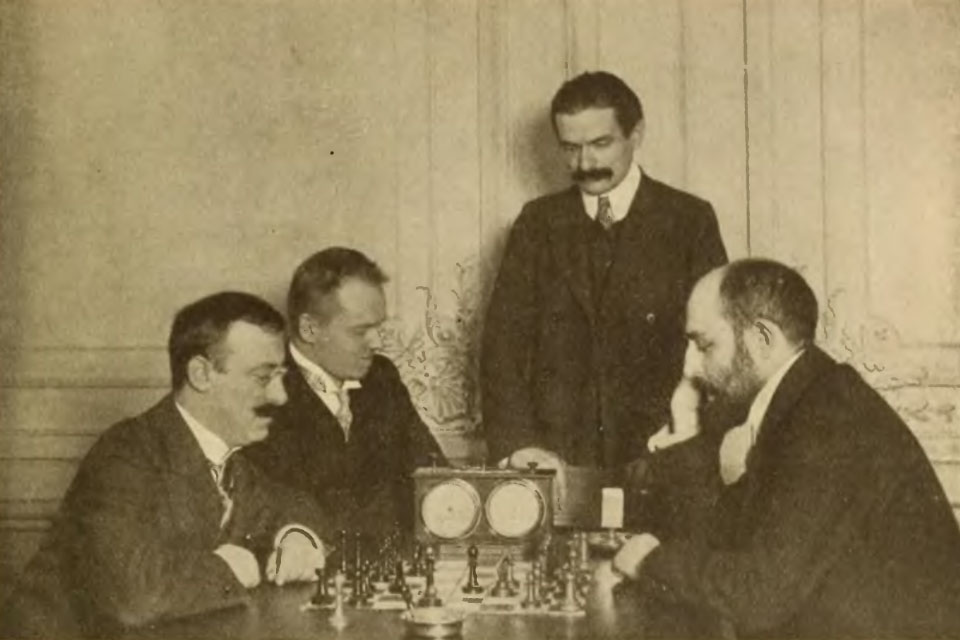
\includegraphics[width=\textwidth]
{img/i4_mieses-bernstein.jpg}\\
\small\sc
j.~mieses \hspace{5cm} dr o.~s.~bernstein
\end{figure}
%%%%%%%%%%%%%%%%


\item There is a time limit of two and one half hours for thirty-seven moves, after that one and one half hours for twenty-three moves, and further on fifty moves an hour. A player transgressing on the time limit loses the game. At the commencement of the game the clock is set in motion. In case a player does not come before the control of time his game is counted as a loss to him.

If a participant fails to appear for the playing of three consecutive games he is removed from the tournament. If such a player has finished less than one half of his games they are not counted; but if he has played more than half of his games, those that he has played are counted and those that he has failed to play are credited to his opponent.

Note to paragraphs 8 and 9: The time of adjournment and the moment of controlling the time can be changed if the majority of participants so desire (As a matter of fact no change was requested.)

\item Either of the players has to carefully write his game and to deliver his manuscript immediately after termination or adjournment of his game to the director of the tournament. All games of the tournament are the property of the St.~Petersburg Chess Club.

\item The participants are forbidden to analyse the games in progress.

\item The tourney is played according to the Chess Year Book by Berger. None of the participants has a right to pardon transgression of these rules by his opponent. Players who do not obey the rules of the tournament, or those who do not complete the tournament, lose every claim to prize, compensation, and their deposit. All differences are settled by the Court of Referees. This Court is composed one half by the participants and one half by the members of the committee. In case the votes are evenly divided, that of the president decides.

%%%%%%%%%%%%%%%%
\begin{figure}[h]
\centering
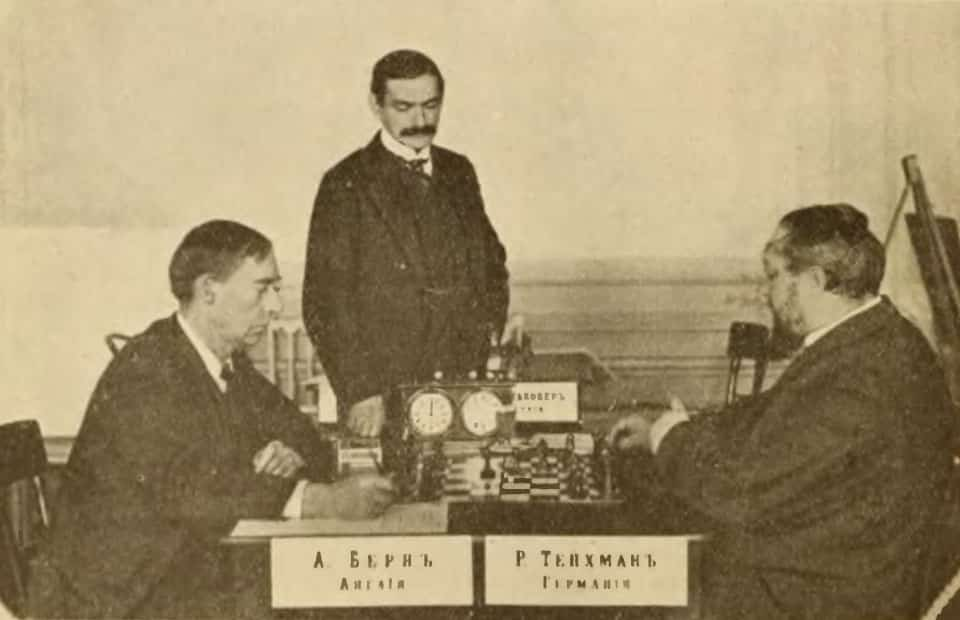
\includegraphics[width=\textwidth]
{img/i5_burn-teichmann.jpg}\\
\small\sc
amos burn \hspace{5cm} r.~teichmann
\end{figure}
%%%%%%%%%%%%%%%%

%%%%%%%%%%%%%%%%
\begin{figure}[h]
\centering
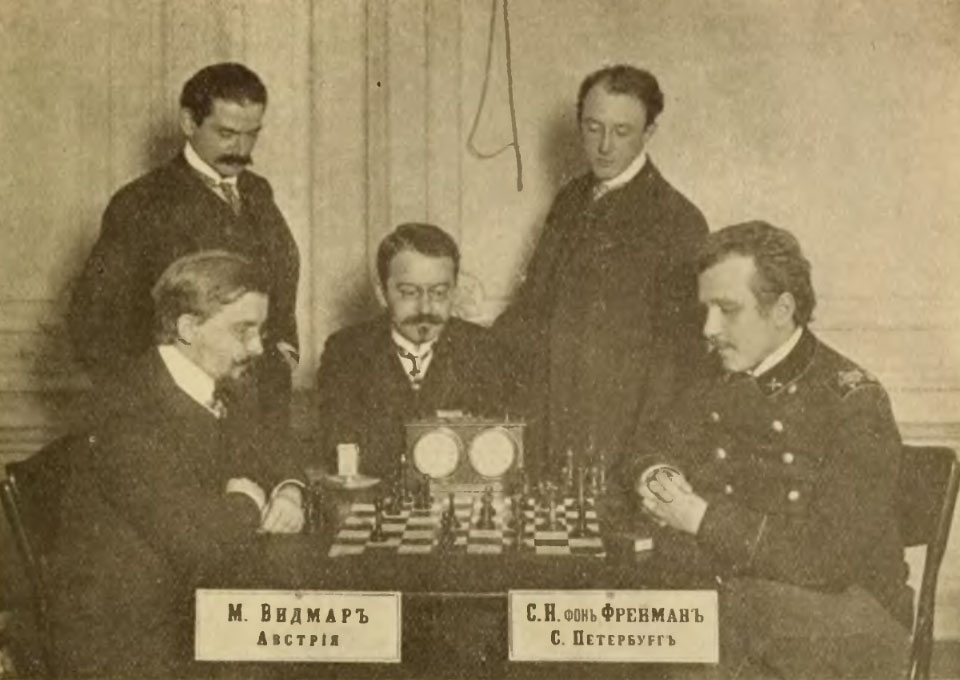
\includegraphics[width=\textwidth]
{img/i6_vidmar-vonfreymann.jpg}\\
\small\sc
m.~vidmar \hspace{5cm} s.~n.~von Freymann
\end{figure}
%%%%%%%%%%%%%%%%

\item On Sunday, the 14th of February, 1909, at 8 o'clock in the evening, the guests will he officially bidden welcome and lots will be drawn for the tournament. The commencement of the tournament is on Monday, the 15th of February, at 11 o'clock A.M.

\item Offers to participate have to be directed no later than the 28th of January, 1909, to the president of the committee of the St.~Petersburg Chess Club, Mr.~P.~P.~Saburow, St.~Petersburg, Mochowaja 27.

\item Participants who desire to have board and lodging at moderate prices are asked to address themselves to the member of the Committee, Mr.~Julius Sossnitsky, St.~Petersburg, Ertelew Perulok 2.
\end{enumerate}

These were the Masters who competed and the countries which they represented: 1. America, Dr.~E.~Lasker; 2. Germany, E.~Colin, J.~Mieses, R.~Spielmann, R.~Teichmann; 3. England, A.~Burn; 4. Holland, A.~Speijer; 5. Austria, Dr.~J.~Perlis, C.~Schlechter, S.~Tartakower, M.~Vidmar; 6. Russia, Dr.~O.~S.~Bernstein, F.~J.~Dus--Chotimirski, S.~N.~von Freymann, W.~J.~Nenarokov, A.~K.~Rubinstein, G.~F.~Salwe, Eugene A.~Znosko-Borovsky; (Carl Rosenkranz retired from the tournament in order to enable Dr.~Perliswho was by chance at St.~Petersburg, to participate); 7. Bohemia, O.~Duras; 8. Hungary, L.~Forg\'acs.\\
\vspace{0.2cm}\\
His Majesty the Czar Nikolaus deigned to give 1000 Rbls.~to strengthen the means at the disposal of the Congress and to donate also a magnificent vase of the Imperial porcelaine manufacture as a first prize tor the all Russian Minor Tournament. The whole amount needed for the Congress, 10,500 Rbls., was gotten together in the way of voluntary contributions.

%%%%%%%%%%%%%%%%
\begin{figure}[h]
\centering
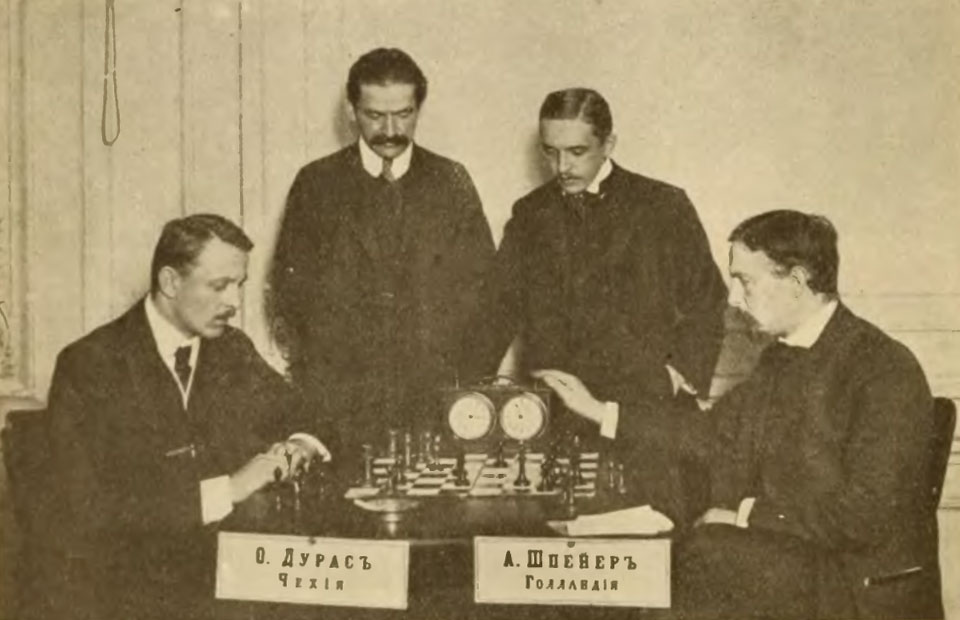
\includegraphics[width=\textwidth]
{img/i7_duras-speijer.jpg}\\
\small\sc
o.~duras \hspace{5cm} a.~speijer
\end{figure}
%%%%%%%%%%%%%%%%